\section{Results}
\label{sec:results}

The numerical results for the problem described in Section \ref{sec:requests} are reported in the following.

\begin{figure}[H]
    \centering
    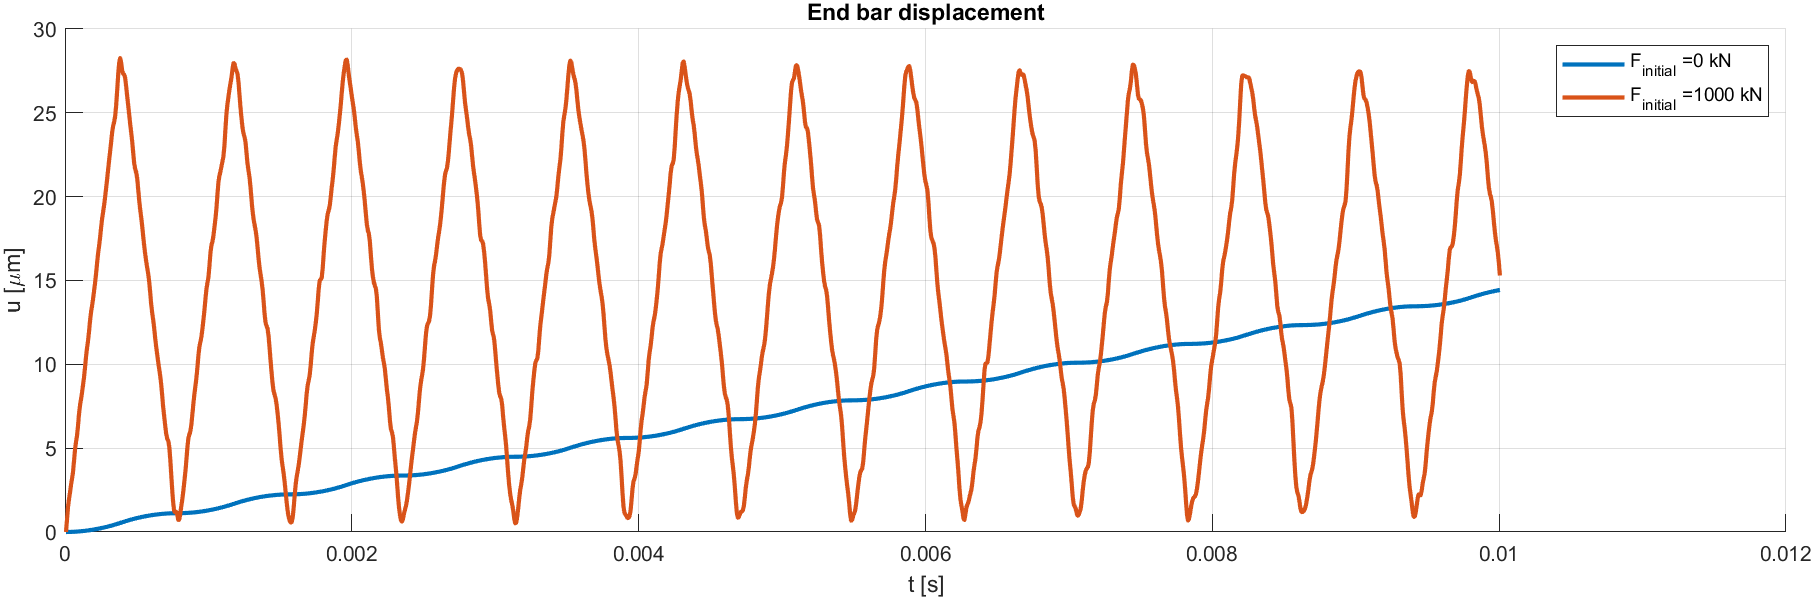
\includegraphics[width=\textwidth]{img/end_bar_displacement_2.png}
    \caption{Displacement of the right end of the bar vs. time}
    \label{fig:final_displacement}
\end{figure}

In Figure \ref{fig:final_displacement} we can observe the displacement of the right end of the bar as a function of time for different values of the initial load $F_{initial}$.
In particular, as also the legend suggests, the plot represents:

\begin{itemize}
    \item Blue curve: $F_{initial} = 0$, $F_{final} = 1000kN$ (linearly increased with respect to time)
    \item Orange curve: $F_{initial} = F_{final} = 1000kN$ (constant)
\end{itemize}

It's easy to see the different behavior of the two cases.

The application of a linearly increasing load (so without discontinuities at the beginning) leads to a displacement that is almost linear in time.
The small oscillation behavior is due to inertia and discretization of the mass distribution along the bar.

On the other hand, the application of a constant load (but with a strong discontinuity at the beginning) leads to a displacement that is definitively not linear (or constant) in time.
The oscillatory behavior is dominant with respect to the previous case and the increasing trend is not as clear as before.


\paragraph{Displacement along the bar}

Another interesting metrics to analyze is the displacement along the bar at different times.

In particular, from Figures \ref{fig:displacement_F0} \& \ref{fig:displacement_F1000} we can observe the displacement of the structure node of the bar at $7$ different times with different loads applied.

\begin{figure}[H]
    \centering
    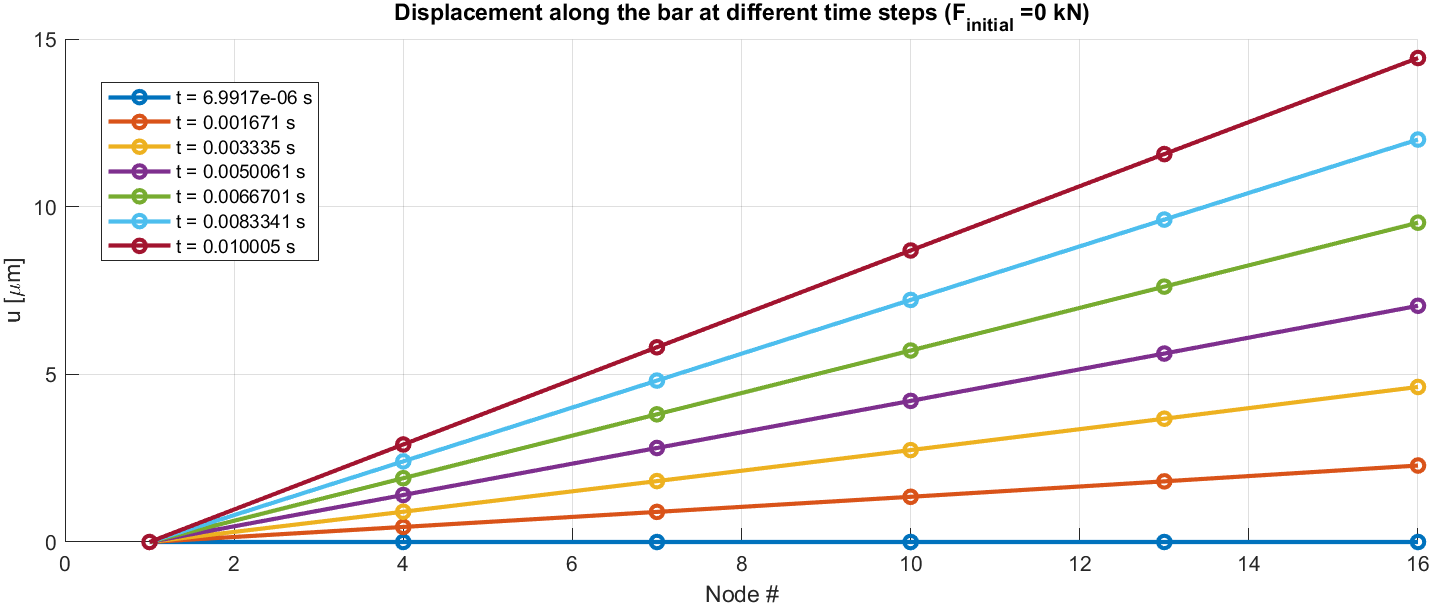
\includegraphics[width=0.8\textwidth]{img/displacement_F0.png}
    \caption{Displacement of the nodes at different times when $F_{initial} = 0 kN$}
    \label{fig:displacement_F0}
\end{figure}

\begin{figure}[H]
    \centering
    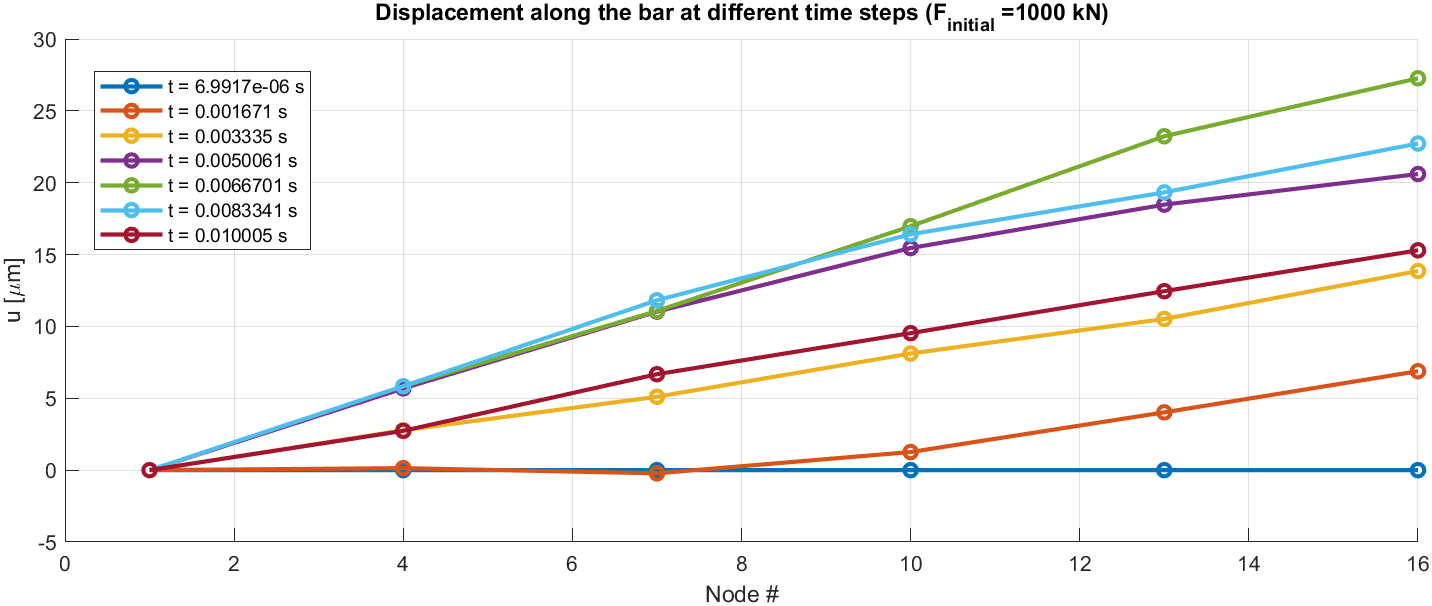
\includegraphics[width=0.8\textwidth]{img/displacement_F1000.png}
    \caption{Displacement of the nodes at different times when $F_{initial} = 1000 kN$}
    \label{fig:displacement_F1000}
\end{figure}

Also from these plots, we can observe the different behavior of the system when different loads are applied.

In case of $F_{initial} = 0 kN$, the displacement is almost linear both in time and in space (displacement lines increase linearly from left to right and from bottom to top).

In case of $F_{initial} = 1000 kN$, the displacement is not linear neither in time nor in space (displacement lines at different times intersects each other which means that the displacement of a given node is not monotonically increasing with time even if the applied load is unidirectional).
This behavior can be explained by the combination of the inertia of the system and the discontinuity in the applied load (wave propagation phenomenon).


\subsection{Parallelism with the mass-spring system}
\label{sub:parallelism_with_the_mass_spring_system}

If we had run the simulation for a longer period, we would have observed that the displacement of the right end of the bar would have reached a constant value, as the contribution of inertia would have gone to zero, finding the equilibrium position governed simply by Hooke's law (since the constitutive law of the material is linear).

Basically, what we are observing in Figure \ref{fig:final_displacement} is just the solution of the following ordinary differential equation (Lagrange's equation) before reaching the equilibrium position or steady state:

\begin{equation}
    \frac{d}{dt} \left( \frac{\partial E_c}{\partial \dot{u}} \right) - \frac{\partial E_c}{\partial u} + \frac{\partial D}{\partial \dot{u}} + \frac{\partial V}{\partial u} = Q
    \label{eq:lagrange_equation}
\end{equation}

Where $E_c$ is the kinetic energy associated with each mass point of the bar, $D$ is the dissipation function which for our problem is considered to be zero, $V$ is the potential energy associated with the elastic deformation of the bar, and $Q$ is the external force applied to the bar.

With this perspective, our rod can be seen as a series of mass points connected by springs, and the solution of our FEM formulation (Figure \ref{fig:final_displacement}) is equivalent to the solution of the equation of motion (Equation \ref{eq:lagrange_equation}) of a system of masses and springs in series.

\begin{figure}[H]
    \centering

    \tikzset{
        spring/.style={thick, decorate, decoration={zigzag, pre length=0.3cm,post length=0.3cm, segment length=6}},
        mass/.style={minimum width=0.6cm, minimum height=0.6cm, draw, outer sep=0pt, thick}
    }

    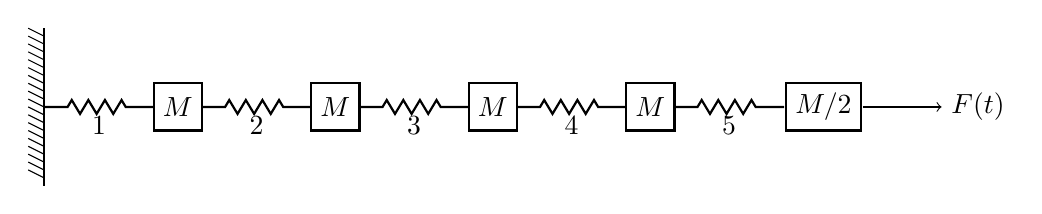
\begin{tikzpicture}

        % Wall
        \draw (-0.2, -1) -- (-0.2,  1);
        \foreach \y in {-.9, -.8, ..., .9}
        \draw (-0.2, \y) -- ++(-0.2, +0.1);

        % Bar
        \foreach \x in {0, 1, ..., 4}
            {
                \draw[spring] (2*\x-0.2, 0) -- ++(2-0.6, 0);
                \node[below] at (2*\x+0.5, 0) {$\the\numexpr\x+1\relax$};
            }

        \foreach \x in {0, 1, ..., 3}
        \node [mass] at (2*\x+1.5, 0) {$M$};

        \node [mass] at (2*4+1.5+0.2, 0) {$M/2$};

        % Force
        \draw[->] (2*4+1.5+0.2+0.5, 0) -- ++(1, 0) node[right]{$F(t)$};

    \end{tikzpicture}
    \caption{System of masses and springs equivalent to the 5 element FEM discretization of the rod with diagonalized mass matrix}
    \label{fig:masses_and_springs}

\end{figure}

In particular, given that we have diagonalized the mass matrix in our FEM formulation, we basically have supposed to move the mass of each FEM element to its extremities.

Notice however the subtle difference between the two systems:

\begin{itemize}
    \item FEM formulation: we are working in a discretized domain, were we are forced to use very small-time steps to capture the dynamics of the system.
    \item Mass-spring system: we are working in a continuous domain (differentiable), where the solution of the equation of motion is a continuous function of time.
\end{itemize}

